\section{Resultados}
En la presente sección se presentarán los resultados de la ejecución de los experimentos planteados. Se presentarán los resultados tanto de forma tabular como de forma gráfica para cada uno de los casos a evaluar. Cabe aclarar que aunque se hicieron 10 repeticiones para ambos algoritmos, en esta seción de resultados solamente se va a presentar el promedio de las 10 repeticiones. \\

\subsection{Tablas de resultados}
A continuación, se presentará una tabla que contiene los promedios de los resultados obtenidos al ejecutar el programa para encontrar la pareja de puntos más cercana en ambos algoritmos 10 veces. Se tuvieron en cuenta principalmente 3 valores en los resultados, los cuales son el tamaño del conjunto de datos de entrada, el tiempo de ejecución del programa y el número de iteraciones realizadas en el programa. Los resultados se pueden encontrar en la tabla 1.\\

\begin{table}[!htbp]
    \centering
    \begin{tabular}{|l|l|l|l|l|}
    \hline
        ~ & \multicolumn{2}{|c|}{Brute force algorithm} & \multicolumn{2}{|c|}{Recursive algorithm} \\ \hline
        size & avg\_time & avg\_iterations & avg\_time & avg\_iterations \\ \hline
        2 & 4390 & 1 & 1190300 & 3 \\ \hline
        4 & 9520 & 6 & 207490 & 9.6 \\ \hline
        8 & 29260 & 28 & 160890 & 18.9 \\ \hline
        16 & 49380 & 120 & 148100 & 36.5 \\ \hline
        32 & 336860 & 496 & 231300 & 70.8 \\ \hline
        64 & 118580 & 2016 & 163580 & 135.3 \\ \hline
        128 & 336390 & 8128 & 187070 & 271.6 \\ \hline
        256 & 543470 & 32640 & 209760 & 530.8 \\ \hline
        512 & 3023210 & 130816 & 359820 & 1045 \\ \hline
        1024 & 1.04E+07 & 523776 & 1134730 & 2096.4 \\ \hline
        2048 & 3.81E+07 & 2096128 & 506270 & 4152.6 \\ \hline
        4096 & 1.44E+08 & 8386560 & 1436830 & 8284.6 \\ \hline
        8192 & 6.13E+08 & 3.36E+07 & 2310720 & 16586.8 \\ \hline
        16384 & 2.05E+09 & 1.34E+08 & 4976390 & 33179.9 \\ \hline
        32768 & 9.24E+09 & 5.37E+08 & 6967510 & 66338.7 \\ \hline
    \end{tabular}
    \caption{Datos resultantes del experimento para ambos algoritmos}
    \label{fig:my_label}
\end{table}


\subsection{Gráficas de resultados}
En la siguiente sección se procesarán los resultados obtenidos anteriormente mediante un programa de python que utiliza la librería Matplotlib para representar los resultados de una manera gráfica. Se mostrará una gráfica logarítmica para cada uno de los algoritmos que mostrará el orden de la complejidad temporal de estos para entradas de distintos tamaños. A continuación en la figura 3 se muestra la gráfica para el algoritmo de fuerza bruta.\\
\begin{figure}[!htbp]
    \centering
    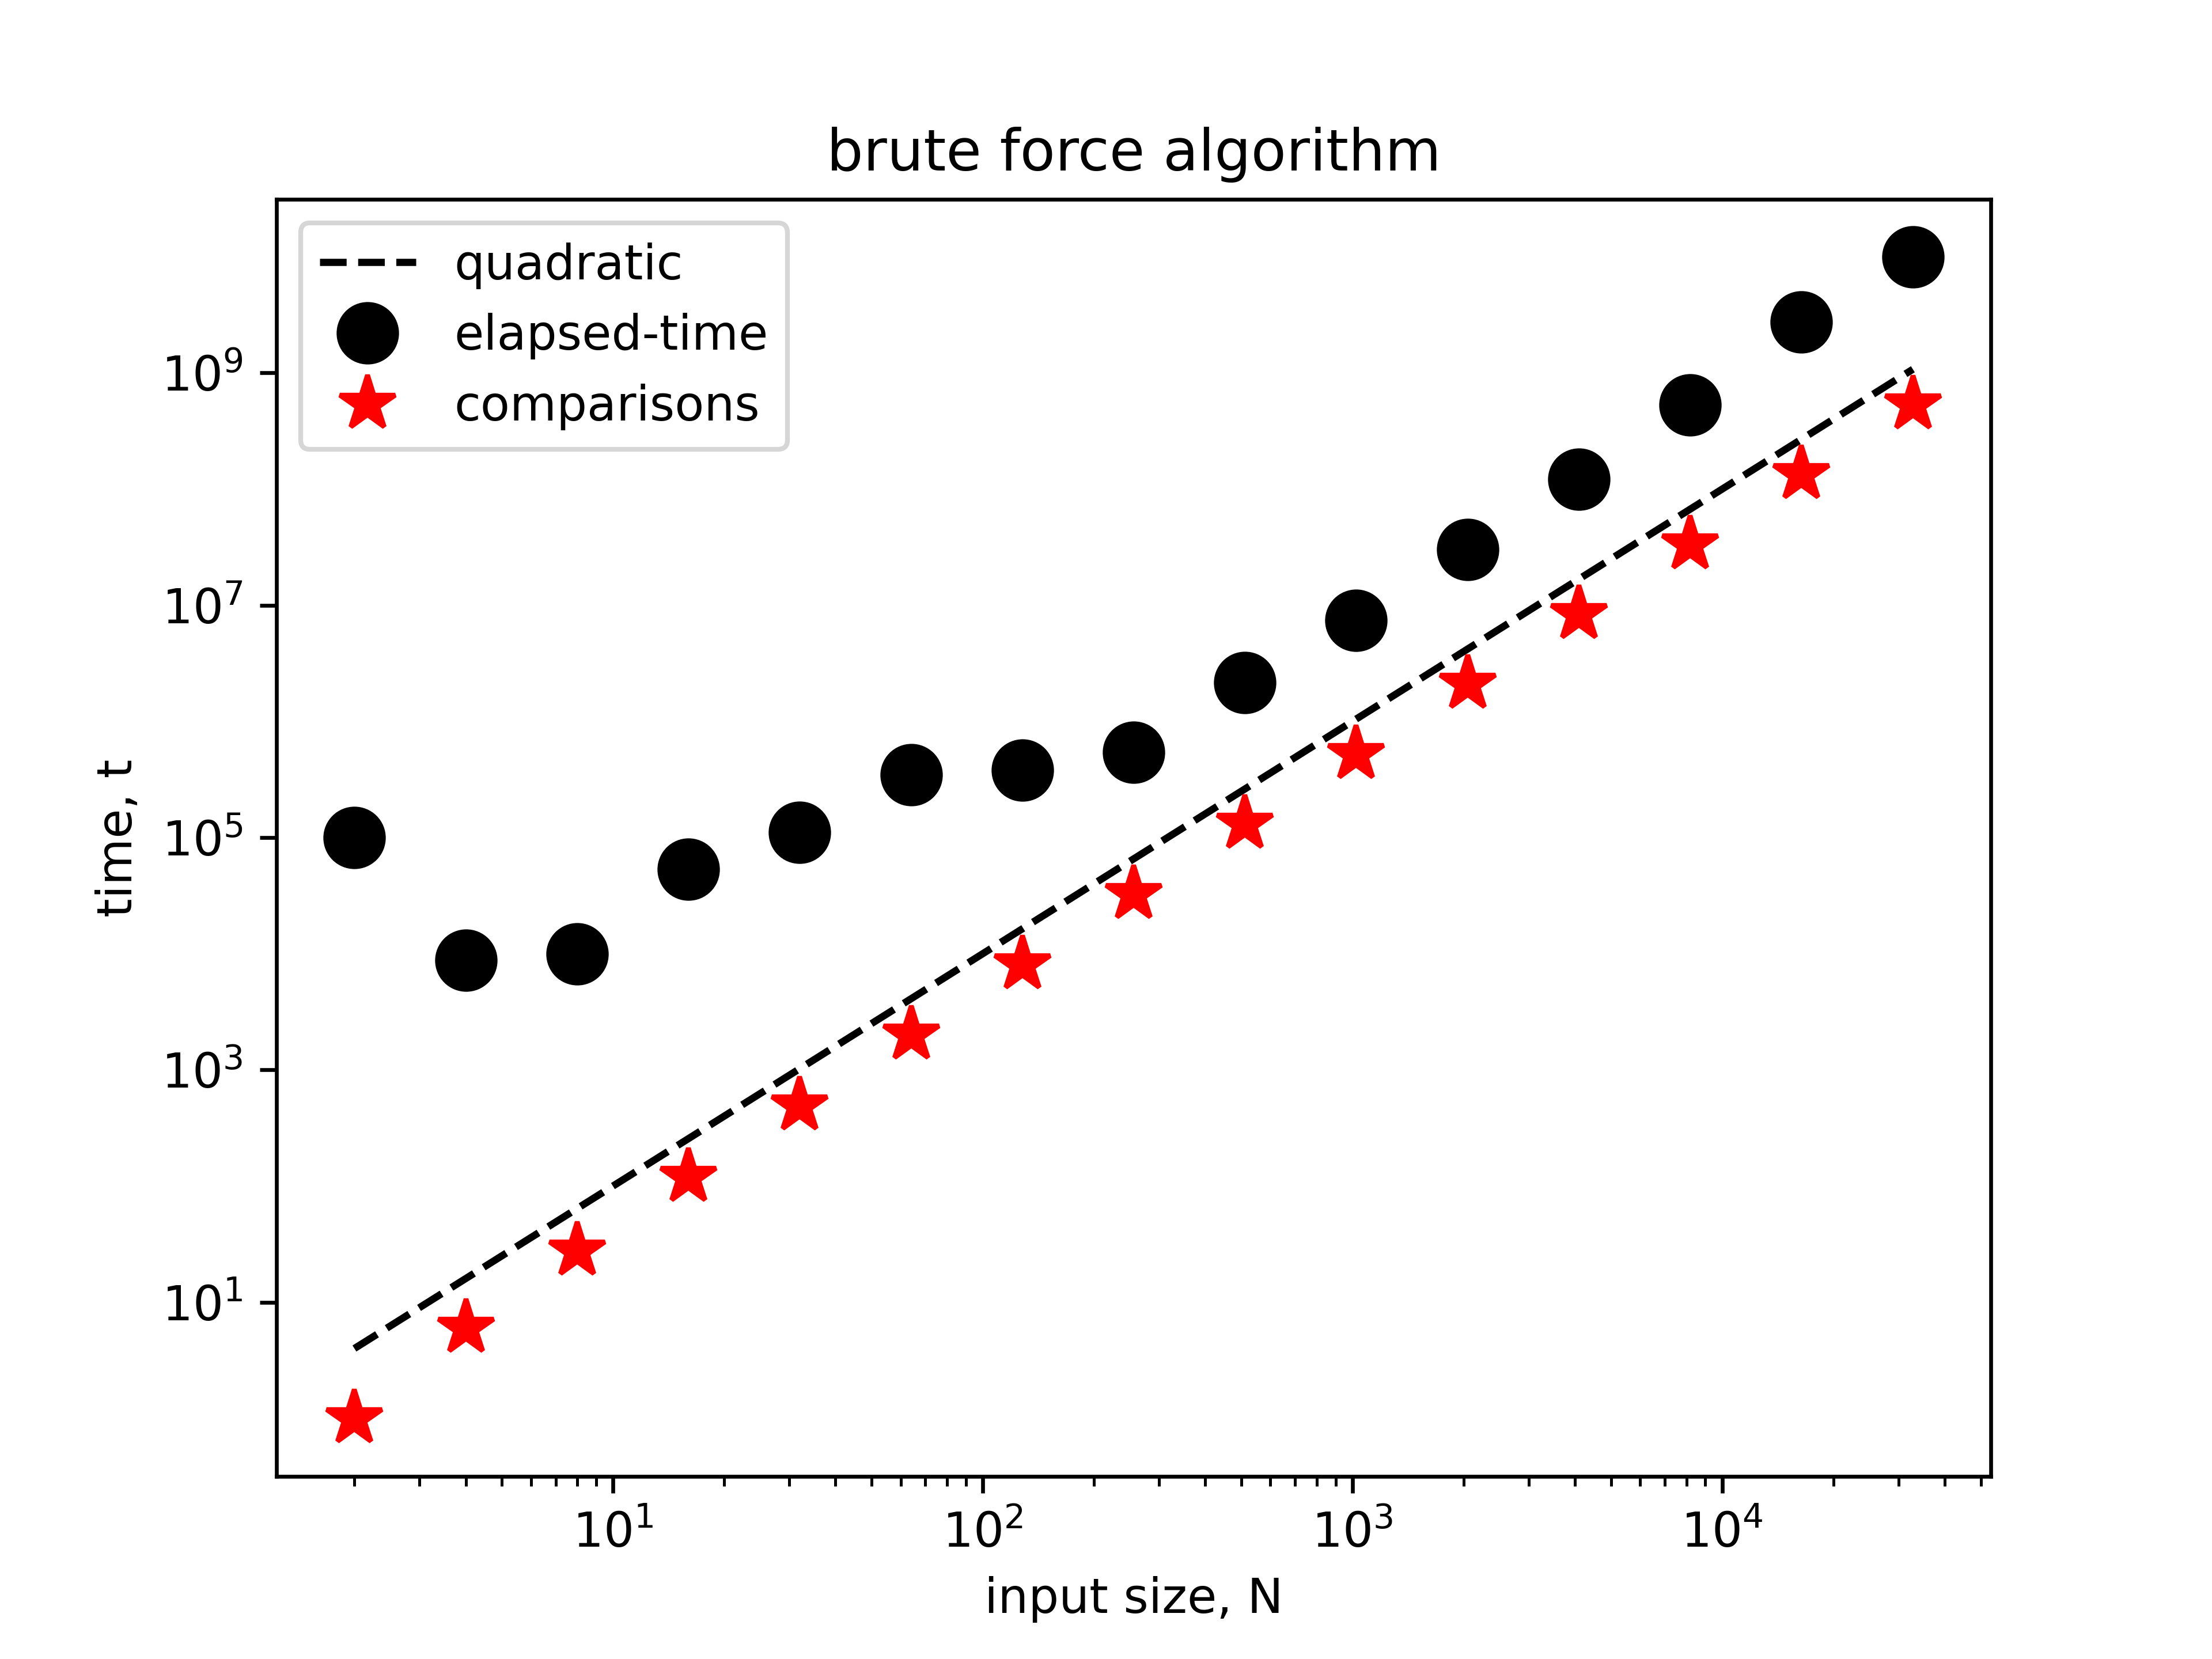
\includegraphics[width=.7\textwidth,height=.5\textwidth]{figures/brute force.png}
    \caption{Gráfica complejidad temporal algoritmo de fuerza bruta}
    \label{fig:my_label}
\end{figure}
La siguiente gráfica es la del algoritmo recursivo. Se puede ver esta en la figura 4.\\
\begin{figure}[!htbp]
    \centering
    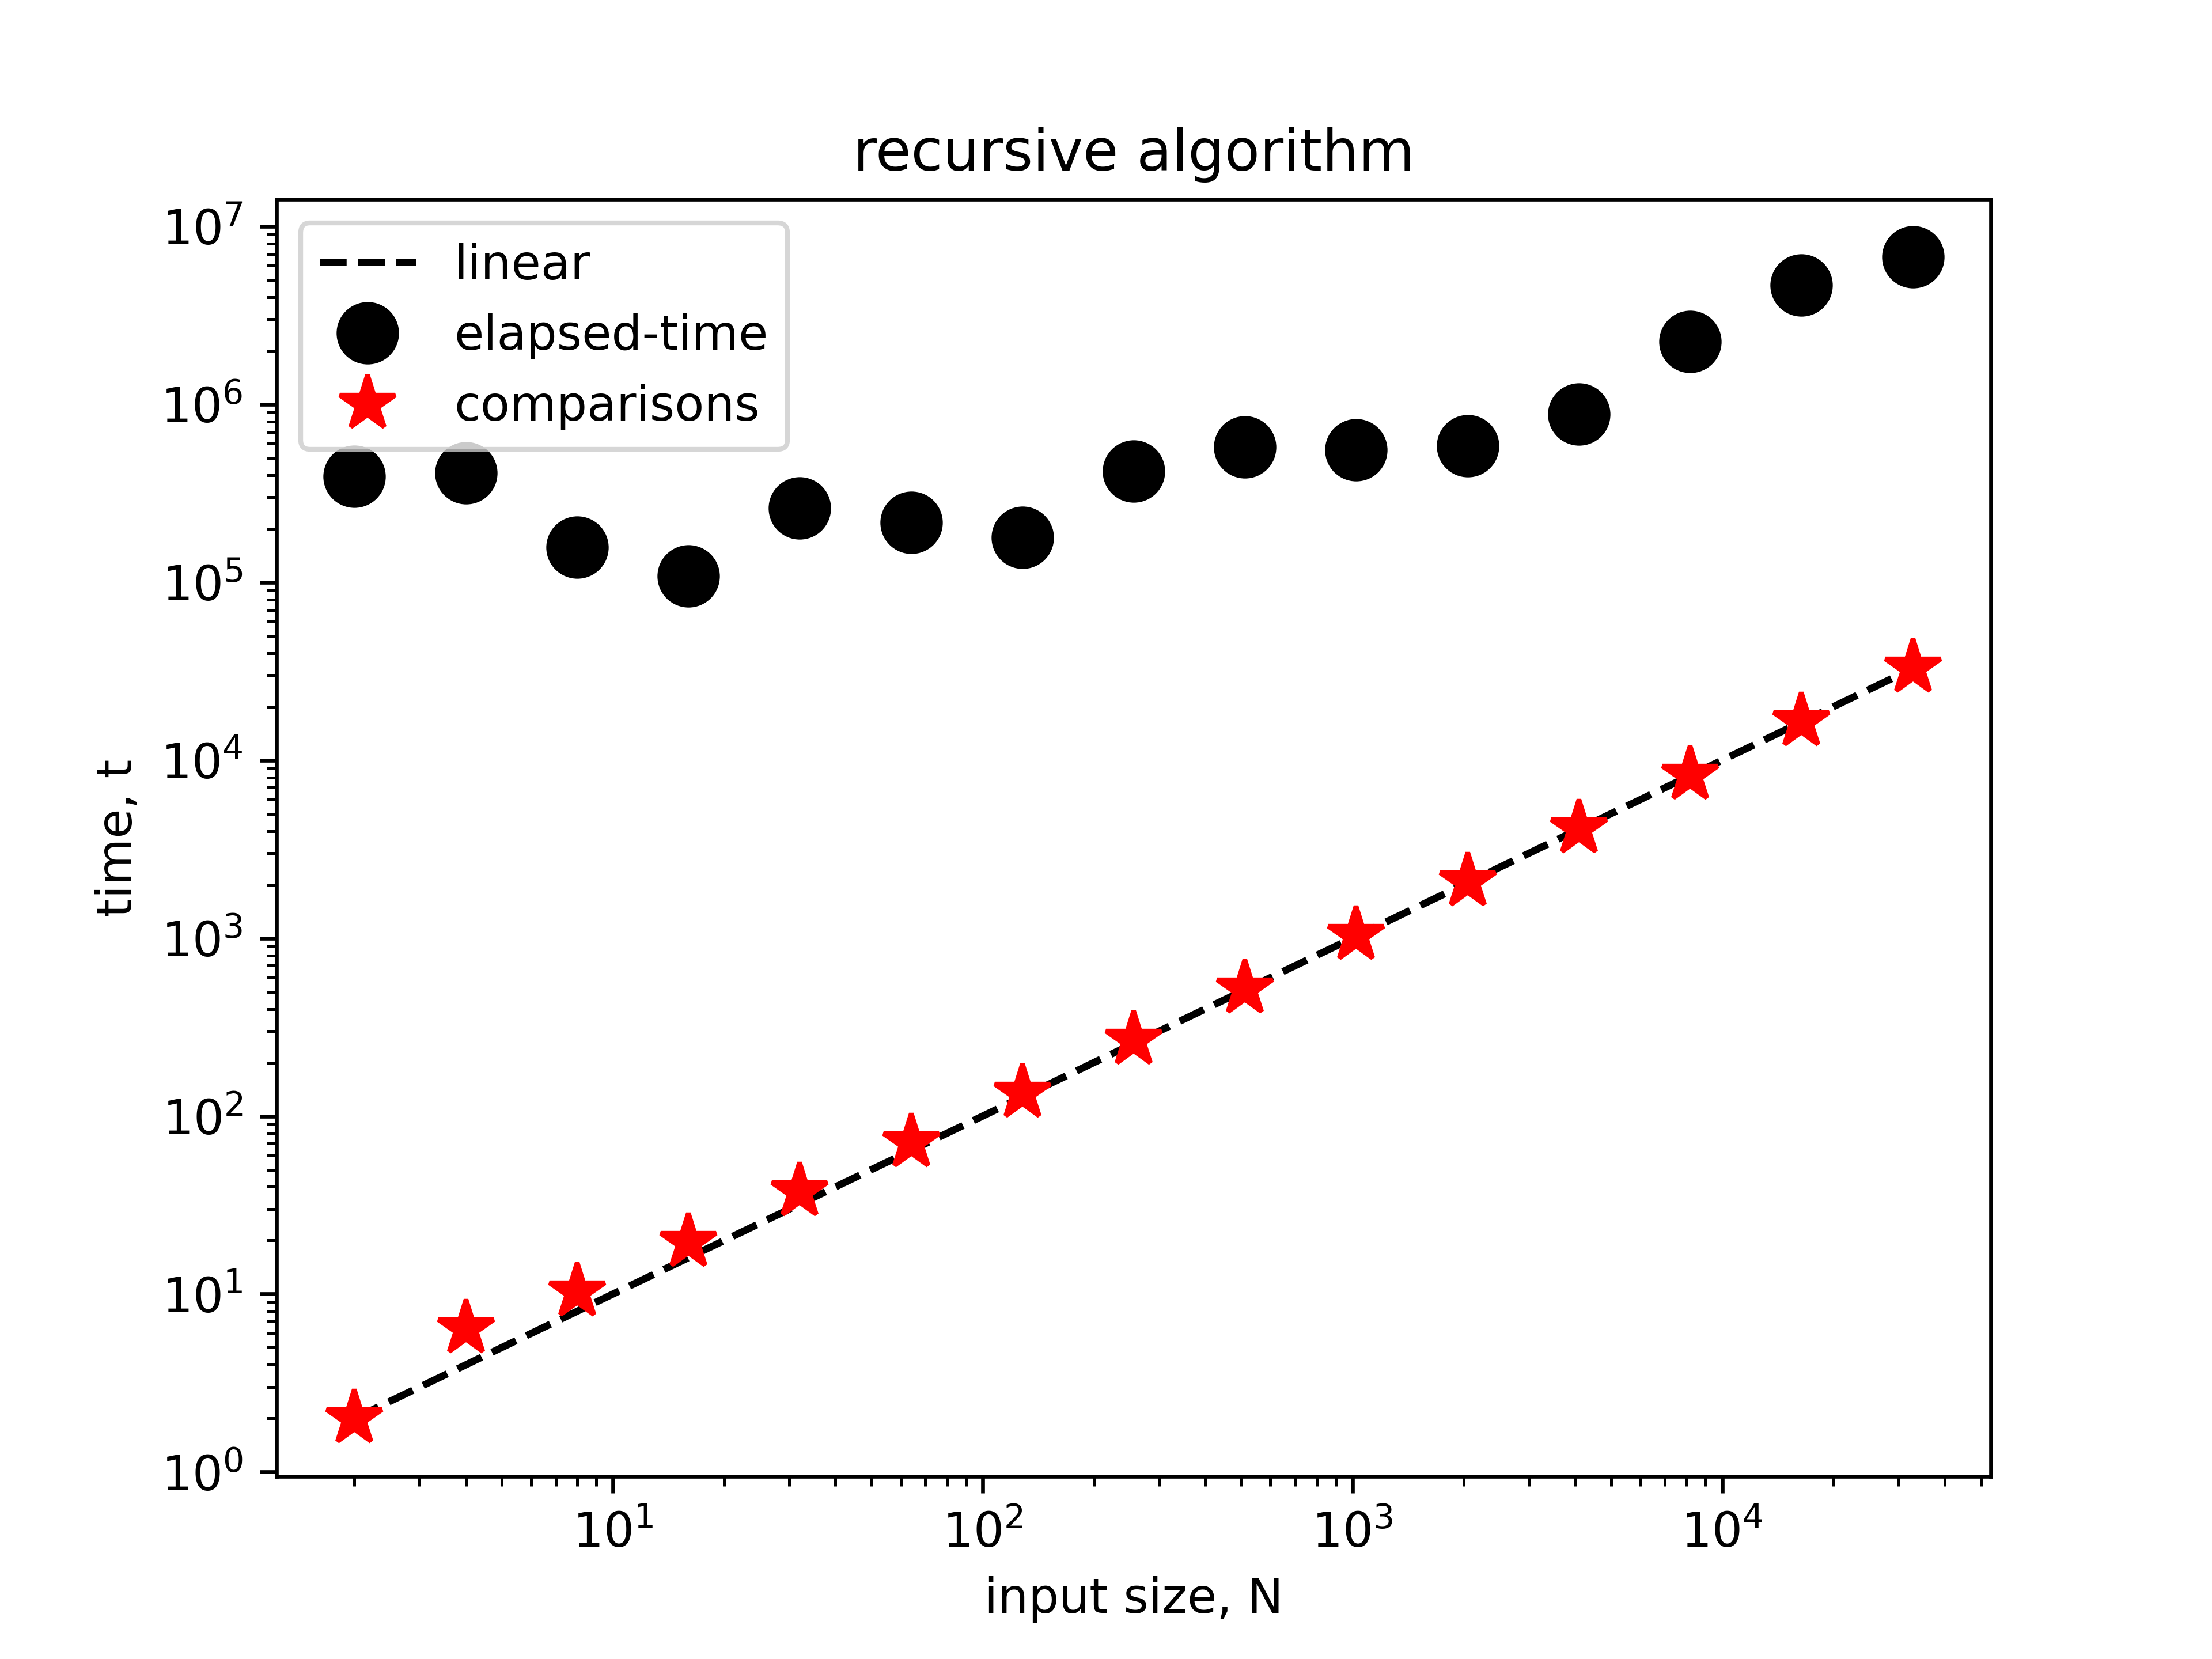
\includegraphics[width=.7\textwidth,height=.5\textwidth]{figures/recursive.png}
    \caption{Gráfica complejidad temporal algoritmo recursivo}
    \label{fig:my_label}
\end{figure}